\documentclass[]{article}
\usepackage[UTF8]{ctex}
\usepackage[a4paper,left=10mm,right=10mm,bottom=10mm,top=10mm]{geometry}
\usepackage{graphicx}
\usepackage{float}
\usepackage{amsmath,amsfonts,amssymb,amsthm}
\usepackage{array,color}
%opening
\title{计算机科学中的数学基础Exercise19}
\author{陈昱衡 521021910939}
\date{\today}
\begin{document}
\maketitle


\section{Basics10}
\begin{figure}[H]
    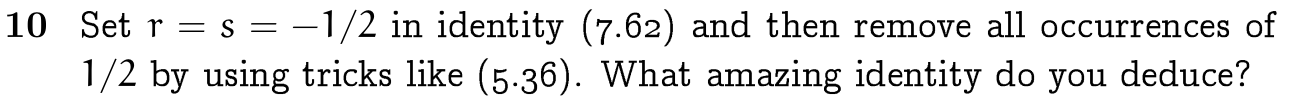
\includegraphics[scale = 0.3]{2023-05-06-17-43-50.png}
\end{figure}
\par 
7.62中的等式:
\begin{figure}[H]
    \centering
    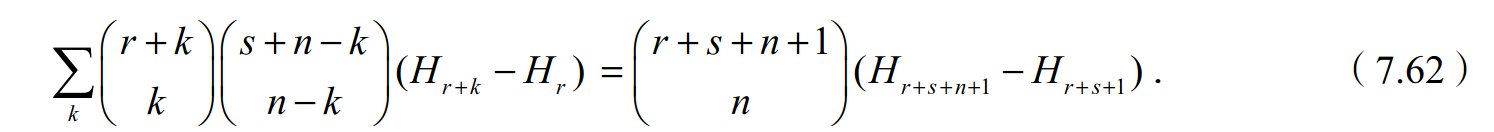
\includegraphics[scale = 0.3]{2023-05-06-17-01-28.png}
\end{figure}
\par 
令$r=s=-\frac{1}{2}$,有
\begin{equation}
    \sum_{k}\binom{k-\frac{1}{2}}{k}\binom{n-k-\frac{1}{2}}{n-k}(H_{k-\frac{1}{2}} - H_{-\frac{1}{2}}) = \binom{n}{n}(H_{n}-H_{0})
\end{equation}
利用5.36中的技巧,即
\begin{figure}[H]
    \centering
    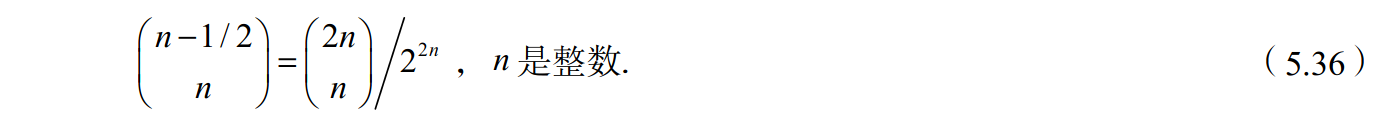
\includegraphics[scale = 0.3]{2023-05-06-17-50-44.png}
\end{figure}
有,
\begin{align}
    &\sum_{k}\binom{2k}{k}\frac{1}{2^{2k}}\binom{2n-2k}{n-k}\frac{1}{2^{2(n-k)}}(H_{k-\frac{1}{2}}-H_{-\frac{1}{2}}) = H_{n}\\
    &\sum_{k}\binom{2k}{k}\binom{2n-2k}{n-k}\frac{1}{2^{2n}}(H_{k-\frac{1}{2}} - H_{-\frac{1}{2}}) = H_{n} 
\end{align}
将$H_{k-\frac{1}{2}} - H_{-\frac{1}{2}}$展开,有:
\begin{align}
    H_{k-\frac{1}{2}} - H_{-\frac{1}{2}} &= \frac{1}{k - \frac{1}{2}} + \frac{1}{k - \frac{3}{2}} + \frac{1}{k - \frac{5}{2}} + \cdots + \frac{1}{1-\frac{1}{2}}\\
    &=\frac{2}{2k-1} + \frac{2}{2k-3} + \frac{2}{2k-5} + \cdots + \frac{2}{1}\\
    &=2H_{2k} - H_{k}
\end{align}

所以,带入整理有
\begin{align}
    \sum_{k}\binom{2k}{n}\binom{2n-2k}{n-k}(2H_{2k} - H_{k}) = 4^n H_{n}
\end{align}


\section{Basics11}
\begin{figure}[H]
    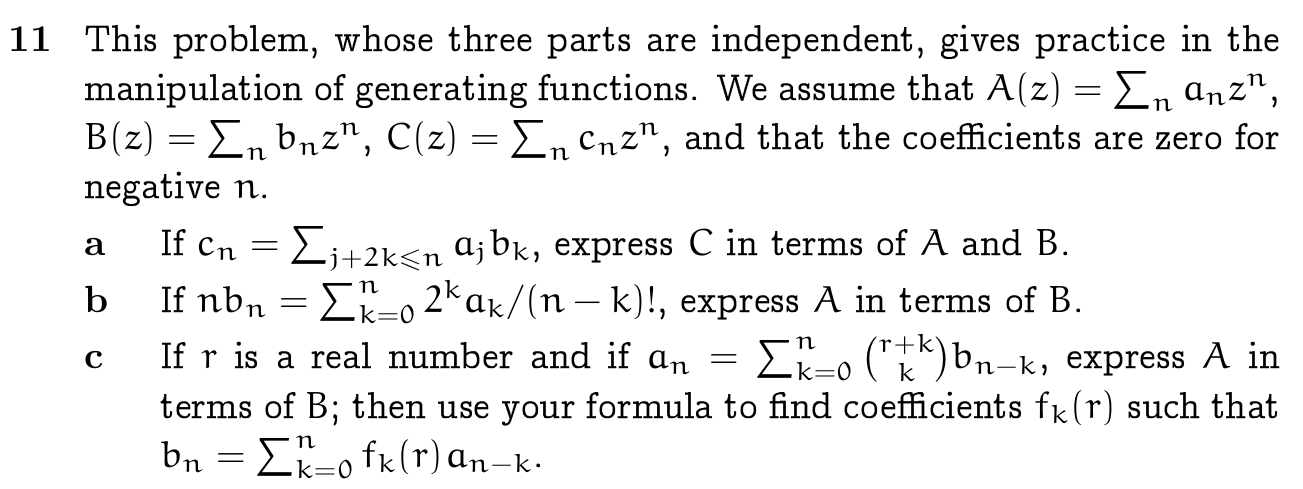
\includegraphics[scale = 0.3]{2023-05-06-17-45-41.png}
\end{figure}
本题中的三个小问,只要根据卷积的形式,根据系数的形式找到对应的生成函数,然后进行卷积即可.\par 
\subsection*{a}
观察系数,由于限制条件为$j + 2k \le n$,而$k$对应的系数为$b_{k}$,如果盲目进行平方,回导致系数不统一。因此,在$B$的生成函数中,可以带入$z^2$。\par 
于是有,
\begin{align}
    A(z)[z^{j}] &= a_jz^j\\
    B(z)[z^{2k}] &= b_kz^{2k}\\
\end{align}
% 将$A$,$B$进行卷积,有
% \begin{align}
%     C(z)[z^n] &= c_nz^n\\
%     &=\sum_{j+2k\le n}a_jb_kz^n\\
%     &=\sum_{j+2k\le n}a_jz^jb_kz^{2k}\\
% \end{align}

因为
\begin{align}
    C(z)[z^n] &= c_nz^n\\
    &=\sum_{0 \le m \le n} \sum_{j+2k\le m}a_jb_kz^n\\
\end{align}

故还需要卷积一个生成函数$\frac{1}{1-z}$。
将三者进行卷积,有
\begin{align}
    A(z)B(z^2)\frac{1}{1-z}[z^n] &= \sum_{j+2k \le n} a_jb_kz^n\\
    &=c_nz^n\\
\end{align}

故,
\begin{align}
    C(z) &= A(z)B(z^2)\frac{1}{1-z}\\
\end{align}

\subsection*{b}
观察题干中系数的关系等式,可以将$\frac{2^ka_k}{(n-k)!}$拆分为$2^ks_k$和$\frac{1}{(n-k)!}$来进行处理。\par
对于$A$的生成函数,我们需要带入$\frac{z}{2}$。\par 
对于第二部分,已有
\begin{align}
    \sum_{n=0}^{\infty}\frac{z^n}{n!} = e^z
\end{align}
\par 
对于$B$的系数$nb_n$,我们可以利用积分与求导的关系来处理多出来的系数$n$。
\par 
即

\begin{align}
    B^{'}(z)[z^{n-1}] = nb_n z^{n-1}\\
\end{align}
\par 

对$A$和$e^z$进行卷积,有
\begin{align}
    A(2z)e^z[z^n] &= (\sum_{k=0}^{n}\frac{a_k}{(n-k)!}2^k)z^n\\
\end{align}
带入$B$,有
\begin{align}
    zB^{'}(z)[z^n] &= nb_nz^n\\
    &= \sum_{k=0}^{n}\frac{2^ka_k}{(n-k)!}z^n\\
    &= A(2z)e^z[z^n]\\
\end{align}
所以有
\begin{align}
    zB^{'}(z) = A(2z)e^z
\end{align}
所以有
\begin{align}
    A_(z) &= \frac{\frac{z}{2}B^{'}(\frac{z}{2})}{e^{\frac{z}{2}}}\\
    &=\frac{zB^{'}(\frac{z}{2})}{2e^{\frac{z}{2}}}
\end{align}

\subsection*{c}
题干中的系数$\binom{r+k}{k}$对应的生成函数是$\frac{1}{(1-z)^{r+1}}$.\par 
因此,有
\begin{align}
    \frac{B(z)}{(1-z)^{r+1}}[z^n] &= \sum_{k=0}^{n}\binom{r+k}{k}b_{n-k}z^n\\
    &=a_n z^{n}\\
    &=A(z)[z^n]\\
\end{align}

所以有
\begin{align}
    A(z) = \frac{B(z)}{(1-z)^{r+1}}
\end{align}

所以,有
\begin{align}
    B(z) &= A(z)(1-z)^{r+1}\\
    A(z)(1-z)^{r+1}[z^n] &= \sum_{k=0}^{n} \binom{r+1}{k}a_{n-k}z^{n-k} \\
    &= \sum_{k=0}^{0}(-1)^k\binom{r+1}{k}a_{n-k}z^{n}\\
\end{align}
所以,有
\begin{align}
    f_{k}(r) = (-1)^k\binom{r+1}{k}
\end{align}

% % \newcommand{\summarize}[2]{Summary of #1: #2}
% % \summarize{Book}{This is a great book.}


% \newcommand{\image}[2]{\begin{figure}[H]\includegraphics[scale = #1]{#2}\end{figure}}

% \image{0.3}{2023-05-06-17-50-44.png}
% \newcommand{\tab}{\begin{table[H]}\centering\begin{tabular}[H]{#1}\end}


\end{document}